\documentclass{rapportPfe}

\usepackage[Lenny]{fncychap} % Ou try Lenny, Bjarne, Glenn, etc.
\usepackage{lipsum}
\usepackage{minted}
\definecolor{bg}{rgb}{0.95,0.95,0.95}

\usepackage{titlesec} % For customizing chapter and section titles
\usepackage{tocloft}  % For customizing the table of contents
\usepackage{hyperref} % For hyperlinks

\title{Système de gestion d'un laboratoire de recherche}

\begin{document}

%----------- Informations du rapport ---------

\titre{Système de gestion d'un laboratoire de recherche}
\sujet{Projet de Fin d'Année}

\enseignant{Khawla \textsc{Asmi}}

\eleves{%
    El Araby \textsc{El Mahdi} \\
    Ossama \textsc{El Khalfi}
}

\jury{%
    Professeur \textsc{Soukaina Bouarourou}
}

%----------- Initialisation -------------------

\fairemarges
\fairepagedegarde

%-------------- Pages préliminaires --------------

\chapter*{Remerciements}
\addcontentsline{toc}{chapter}{Remerciements}
Nous remercions chaleureusement l’équipe pédagogique de l’Université Mohammed V pour son accompagnement durant ce projet. Nos remerciements s’adressent également à notre encadrant pour ses conseils avisés et à nos proches pour leur soutien.

\chapter*{Résumé}
\addcontentsline{toc}{chapter}{Résumé}
Ce rapport présente le développement d’un système centralisé destiné à la gestion d’un laboratoire de recherche, en réponse aux limites des méthodes traditionnelles. L’application permet d’automatiser les processus administratifs, de faciliter la communication entre chercheurs et de renforcer la sécurité des données. Ce travail s’inscrit dans le cadre du projet de fin d’année à l’Université Mohammed V.

\chapter*{Liste des Abréviations}
\addcontentsline{toc}{chapter}{Liste des Abréviations}
\begin{itemize}
  \item \textbf{API} : Application Programming Interface
  \item \textbf{UI} : User Interface
  \item \textbf{DB} : Database
  \item \textbf{CRUD} : Create, Read, Update, Delete
\end{itemize}

\newpage
\chapter*{Introduction générale}
\addcontentsline{toc}{chapter}{Introduction générale}

La gestion d’un laboratoire de recherche moderne représente un défi multidimensionnel, nécessitant une coordination rigoureuse des activités scientifiques, administratives et collaboratives. Les enjeux majeurs incluent l’optimisation des processus de publication, le suivi des participations aux conférences, la facilitation des échanges et la sécurisation des données de recherche.

Actuellement, de nombreux laboratoires recourent à des méthodes de gestion traditionnelles, reposant sur des outils bureautiques non spécialisés (tableurs, messageries électroniques, systèmes de stockage génériques). Bien que ces solutions soient largement répandues, elles présentent des lacunes significatives : redondance des tâches, dispersion des informations, risques d’erreurs et absence de centralisation. Ces limitations entravent la productivité scientifique et compliquent la prise de décision stratégique.

Dans ce contexte, le développement d’une application web dédiée à la gestion des laboratoires de recherche s’impose comme une solution incontournable. Une telle plateforme permettrait d’automatiser les processus répétitifs, de structurer la collaboration et d’assurer une meilleure traçabilité des données, tout en renforçant la sécurité et l’accessibilité de l’information.

\newpage
\tabledematieres

\newpage
\listoffigures

\newpage
\listoftables

%------------ Corps du rapport ----------------

\chapter{Généralités sur le projet}

\section{Problématique}

La gestion efficace d’un laboratoire de recherche repose sur la coordination fluide des activités scientifiques, administratives et humaines. Pourtant, de nombreux laboratoires continuent d’utiliser des approches archaïques, souvent basées sur des outils génériques, peu adaptés à la complexité croissante de la recherche contemporaine. Cette situation engendre de nombreuses limites que nous analysons ci-dessous.

\subsection{Une Gestion Manuelle Fragmentée et Source d’Incohérences}

Les laboratoires s’appuient encore trop souvent sur des solutions non spécialisées comme les tableurs ou les échanges de courriels pour suivre les publications, projets, conférences et collaborations.

\begin{itemize}
  \item \textbf{Suivi imprécis et chronophage} : La saisie manuelle des données entraîne des erreurs fréquentes, une mise à jour fastidieuse et une perte de temps considérable, nuisant à la fiabilité du suivi scientifique.
  \item \textbf{Données dispersées et non structurées} : Les informations sont stockées dans des fichiers multiples et non synchronisés, rendant difficile l’obtention d’une vue d’ensemble cohérente et à jour.
  \item \textbf{Vulnérabilité accrue des données} : L’absence de protocoles robustes de sauvegarde et de sécurité expose les fichiers à des risques de perte, de corruption ou d’accès non autorisé.
\end{itemize}

\subsection{Communication Désorganisée et Collaboration Sous-Exploitées}

La réussite d’un laboratoire dépend de la qualité des échanges entre ses membres. Cependant, les outils de communication utilisés ne sont ni centralisés ni adaptés à un environnement scientifique.

\begin{itemize}
  \item \textbf{Canaux de communication éparpillés} : Entre messageries personnelles et échanges informels, la traçabilité et la conservation des discussions deviennent difficiles.
  \item \textbf{Faible intégration des outils collaboratifs} : L'absence de solutions intégrées et spécialisées freine la coordination et crée des silos informationnels.
\end{itemize}

\subsection{Défauts de Sécurité et Faible Capacité d'Évolution}

Les systèmes traditionnels, souvent construits de manière ad hoc, présentent des failles critiques.

\begin{itemize}
  \item \textbf{Contrôle d’accès rudimentaire} : La gestion des rôles et des permissions est inexistante ou limitée, ce qui compromet la confidentialité des données sensibles.
  \item \textbf{Infrastructure hétérogène et difficile à maintenir} : La coexistence d’outils isolés rend la maintenance complexe, coûteuse et sujette aux pannes.
  \item \textbf{Absence de scalabilité} : Ces systèmes ne sont pas conçus pour évoluer avec l’augmentation du nombre d’utilisateurs, de projets ou du volume de données, limitant leur durabilité.
\end{itemize}

\section{L’objectif à réaliser}

\subsection{Objectif Principal}
Développer une application web centralisée, sécurisée, performante et ergonomique pour optimiser la gestion des laboratoires de recherche. Elle repose sur une architecture à microservices, une base de données PostgreSQL, et un outil d’intelligence artificielle en Python pour résumer automatiquement les publications scientifiques.

\subsection{Fonctionnalités Principales}
\begin{itemize}
  \item \textbf{Suivi des publications et conférences} : Vision synthétique et historique complet, avec génération automatique de résumés via l’IA.
  \item \textbf{Messagerie instantanée} : Communication en temps réel entre les membres.
  \item \textbf{Gestion des droits d’accès} : Permissions avancées selon le rôle (administrateur, chercheur, responsable).
\end{itemize}

\subsection{Objectifs Secondaires}
\begin{itemize}
  \item Automatiser les tâches pour libérer du temps.
  \item Centraliser les échanges et favoriser la collaboration.
  \item Assurer la pérennité, la sécurité et la traçabilité des données.
  \item Créer une solution évolutive et maintenable sur le long terme.
\end{itemize}


\chapter{Spécification des besoins}

L’architecture backend de cette application repose sur une conception modulaire et distribuée, mettant l’accent sur la séparation claire des responsabilités. Cette méthode vise à maximiser la facilité de maintenance, la possibilité d’évolution indépendante des services, ainsi que la robustesse globale du système. Chaque service, dédié à une fonction métier spécifique, est développé avec la technologie la plus appropriée à ses besoins, tout en s’intégrant harmonieusement dans l’ensemble de l’écosystème applicatif.

\section{Service de gestion des publications et conférences : \texttt{Rust}}

Ce service est développé en Rust, en réponse à des exigences strictes de performance, fiabilité et sécurité. Il gère l’ensemble du cycle de vie des publications et conférences à travers des API performantes, incluant un service dédié au téléversement de fichiers ainsi qu’un point de terminaison pour l’observation de métriques internes.

\begin{itemize}
    \item \textbf{Performance et gestion efficace des ressources :} Rust compile en code natif performant, proche du C/C++, sans ramasse-miettes, ce qui est essentiel pour traiter de gros volumes de données bibliographiques et de fichiers.
    \item \textbf{Sécurité mémoire et fiabilité :} Le système d’emprunt de Rust élimine les erreurs mémoire à la compilation, garantissant l’intégrité des données même dans des scénarios à forte charge.
    \item \textbf{Service de téléversement :} Un composant dédié en Rust prend en charge le téléversement sécurisé des fichiers de publication (PDF, documents complémentaires), avec vérification, stockage et association automatique aux métadonnées.
    \item \textbf{Point de terminaison de métriques :} Le service expose un point de terminaison \texttt{/metrics} personnalisé, fournissant des statistiques internes telles que le nombre de téléversements, les temps de réponse, les erreurs rencontrées ou encore l’état des composants, facilitant la supervision et le diagnostic.
    \item \textbf{Gestion avancée de la concurrence :} Grâce au modèle de possession de Rust, le traitement simultané des requêtes est effectué de manière sûre, sans accès concurrent dangereux à la mémoire.
\end{itemize}

Rust s’avère donc particulièrement adapté aux systèmes critiques nécessitant robustesse, performance et observabilité. Il bénéficie également d’un écosystème web moderne (\texttt{Axum}, \texttt{SQLx}, etc.) facilitant la construction d’API web fiables et maintenables.

Rust est donc particulièrement adapté aux systèmes critiques. Il bénéficie par ailleurs d’un écosystème web moderne (\texttt{Axum}, \texttt{SQLx}, etc.) permettant la création d’API web performantes et robustes.

Rust est donc particulièrement adapté aux systèmes critiques. Il bénéficie par ailleurs d’un écosystème web moderne (\texttt{Axum}, \texttt{SQLx}, etc.) permettant la création d’API web performantes et robustes.

Rust est donc particulièrement adapté aux systèmes critiques et bénéficie d’un écosystème web solide pour des API robustes.

\section{Service d’authentification et gestion des identités : \texttt{Node.js} avec \texttt{TypeScript}}

Ce service gère l’authentification avec Node.js et TypeScript, pour combiner rapidité de développement et sécurité.

\begin{itemize}
    \item \textbf{Modèle asynchrone et non bloquant :} Idéal pour les vérifications I/O comme la validation de tokens.
    \item \textbf{Robustesse et maintenabilité :} TypeScript améliore la détection d’erreurs et la lisibilité du code.
    \item \textbf{Écosystème sécurisé :} Utilisation de bibliothèques reconnues telles que \texttt{Passport.js}, \texttt{bcrypt.js}, et \texttt{jsonwebtoken}.
    \item \textbf{Limites et solutions :} Pour des charges cryptographiques spécifiques, des modules natifs peuvent être intégrés.
\end{itemize}

\section{Serveur de communication en temps réel (chat) : \texttt{Node.js} avec WebSockets}

Ce service permet des communications bidirectionnelles en temps réel.

\begin{itemize}
    \item \textbf{WebSockets :} Connexions TCP persistantes et full-duplex pour des échanges instantanés.
    \item \textbf{Scalabilité :} L’event loop de Node.js gère efficacement un grand nombre de connexions. Redis Pub/Sub peut assurer la scalabilité horizontale.
\end{itemize}

\section{Interface utilisateur (frontend) : \texttt{Next.js} avec \texttt{TypeScript}}

Développé avec Next.js (React) pour des performances optimales et une bonne maintenabilité.

\begin{itemize}
    \item \textbf{Performance et SEO :} Rendu côté serveur (SSR) et génération statique (SSG).
    \item \textbf{Cohérence des types :} Partage de définitions TypeScript entre frontend et backend.
    \item \textbf{UX :} Interface responsive et gestion structurée de l’état applicatif.
\end{itemize}

\section{Persistance des données : \texttt{PostgreSQL}}

PostgreSQL est choisi pour sa robustesse, ses performances élevées et son respect strict des standards relationnels.

\begin{itemize}
    \item \textbf{Intégrité des données :} Garantit les propriétés ACID (Atomicité, Cohérence, Isolation, Durabilité) pour assurer la fiabilité des transactions.
    \item \textbf{Fonctionnalités avancées :} Offre un support natif pour les données semi-structurées via \texttt{JSONB}, ainsi que des capacités performantes de recherche en texte intégral.
    \item \textbf{Scalabilité et haute disponibilité :} Intègre des mécanismes de réplication, de partitionnement et de gestion des charges pour répondre aux besoins croissants.
    \item \textbf{Comparaison avec d’autres SGBD :} Préféré à des bases NoSQL comme MongoDB lorsqu’il s’agit de gérer des contraintes relationnelles complexes et des opérations transactionnelles strictes.
\end{itemize}

\section{ORM pour base de données : \texttt{Prisma} avec \texttt{TypeScript}}

Utilisé dans le backend d’authentification pour faciliter l’accès à la base de données PostgreSQL.

\begin{itemize}
    \item \textbf{Simplicité :} Schéma déclaratif, génération automatique de clients typés.
    \item \textbf{Type-safety :} Autocomplétion, détection d’erreurs.
    \item \textbf{Sécurité :} Prévention des injections SQL via requêtes typées.
    \item \textbf{Transactions :} Support robuste avec gestion concurrente optimisée.
\end{itemize}

\section{Conteneurisation et orchestration : \texttt{Docker}}

Tous les services, y compris la base de données et les données mock, sont conteneurisés grâce à Docker et orchestrés avec Docker Compose.

\begin{itemize}
    \item \textbf{Isolation complète :} Chaque service s’exécute dans un environnement indépendant, garantissant une isolation des processus et des dépendances.
    \item \textbf{Portabilité et cohérence :} Les conteneurs peuvent être déployés sans modification sur des serveurs locaux, des environnements cloud, ou des clusters.
    \item \textbf{Réseau flexible :} Gestion des adresses IP internes pour la communication inter-services, ainsi que des IP externes pour l’accès public contrôlé.
    \item \textbf{Données mock intégrées :} Les données de test sont préchargées via des conteneurs dédiés pour faciliter le développement et les tests.
    \item \textbf{Préparation à l’orchestration avancée :} La configuration est conçue pour une migration future vers Kubernetes, facilitant l’évolution et la montée en charge.
\end{itemize}

\newpage
\section{Intégration d'une intelligence artificielle : \texttt{Python}}

Python est utilisé pour le développement des modules d’intelligence artificielle grâce à son écosystème riche et ses bibliothèques avancées de traitement du langage naturel.

\begin{itemize}
    \item \textbf{API web performante :} Utilisation de FastAPI pour exposer des API RESTful et gérer des connexions WebSocket, assurant une communication réactive et scalable.
    \item \textbf{Traitement avancé des documents :} Extraction et analyse de contenu PDF pour alimenter les modèles d’IA.
    \item \textbf{Modèles de NLP :} Implémentation de modèles pré-entraînés de génération et résumé automatique de texte, appuyée par des techniques de tokenisation et prétraitement linguistique.
    \item \textbf{Interopérabilité et maintenabilité :} Architecture modulaire facilitant l’intégration avec les autres composants du système et simplifiant la maintenance.
\end{itemize}

\section*{Conclusion}

L’architecture modulaire adoptée, fondée sur des microservices spécialisés, est conçue pour répondre à des exigences élevées de performance, de fiabilité et d’évolutivité. Chaque composant est isolé, facilitant la maintenance, la mise à jour, et la résilience du système. Cette approche permet aussi une intégration continue de nouvelles technologies, assurant la pérennité de la plateforme.


\section{Comparaison des Architectures : Monolithique vs Microservices}

L’architecture générale de l’application adopte un modèle hybride. Les fonctionnalités principales (gestion des publications, authentification, etc.) reposent sur une architecture microservices, tandis que le serveur de messagerie instantanée est développé selon une structure monolithique. Cette section présente une comparaison critique entre ces deux paradigmes, dans le contexte spécifique de notre système.

\subsection{Tableau comparatif des caractéristiques}

\begin{center}
\begin{tabular}{|p{4cm}|p{5.5cm}|p{5.5cm}|}
\hline
\textbf{Critère} & \textbf{Microservices (Cœur de l'application)} & \textbf{Monolithique (Serveur de chat)} \\
\hline
Organisation du code & Services indépendants (Rust, Node.js, Python) & Code unifié dans un seul bloc (Node.js + WebSockets) \\
\hline
Scalabilité & Évolutivité horizontale par service & Évolutivité verticale via une instance unique \\
\hline
Déploiement & Déploiement autonome de chaque service (Docker) & Déploiement unique en un seul paquet \\
\hline
Complexité & Complexité accrue (réseau, orchestration) & Complexité initiale réduite \\
\hline
Performance & Optimisation spécifique à chaque service & Faible latence pour les traitements en temps réel \\
\hline
Cohérence des données & Cohérence éventuelle (transactions distribuées complexes) & Cohérence forte (base de données unique) \\
\hline
Liberté technologique & Technologies variées selon le besoin & Restreinte à l’écosystème Node.js \\
\hline
Isolation des pannes & Défaillances circonscrites à un seul service & Risque de panne globale en cas de crash \\
\hline
Vitesse de développement & Autonomie par équipe/service & Rapidité dans un environnement centralisé \\
\hline
\end{tabular}
\end{center}

\subsection{Choix des microservices pour le cœur applicatif}

\begin{enumerate}
    \item \textbf{Adaptation technologique par domaine} : Chaque composant est développé avec le langage ou l’environnement le plus adapté à ses exigences spécifiques. \\
    \textit{Exemple :} Rust pour les opérations performantes sur fichiers ; Node.js pour la gestion asynchrone des sessions.
    
    \item \textbf{Scalabilité ciblée} : Les composants fortement sollicités, tels que l’API Gateway, peuvent être mis à l’échelle indépendamment, sans impacter les autres services.
    
    \item \textbf{Facilité de maintenance} : Les séparations logiques entre les services (par domaine fonctionnel) facilitent la gestion, le débogage et les évolutions futures.\\
    \textit{Exemple :} Aucun modèle de données n’est partagé entre les modules d’authentification et de publication.
    
    \item \textbf{Résilience accrue} : En cas de panne dans un service (ex. : service des publications), les autres continuent de fonctionner normalement (ex. : authentification).
\end{enumerate}

\subsection{Justification du choix monolithique pour le serveur de chat}

\begin{enumerate}
    \item \textbf{Contraintes de temps réel} : WebSocket repose sur une communication bidirectionnelle à faible latence, difficile à reproduire entre services séparés par un réseau.
    
    \item \textbf{Gestion d’état centralisée} : Le suivi des connexions actives, des messages et des statuts de présence est simplifié dans une architecture monolithique.
    
    \item \textbf{Rapidité de développement} : Les fonctionnalités interdépendantes (ex. : statut + messagerie) sont plus rapides à développer dans un code unique et intégré.
    
    \item \textbf{Optimisation des performances} : L’absence de latence réseau entre composants internes améliore la réactivité des échanges instantanés.
\end{enumerate}

\subsection{Enjeux identifiés et stratégies d’atténuation}

\begin{center}
\begin{tabular}{|p{4.5cm}|p{5cm}|p{5cm}|}
\hline
\textbf{Problème identifié} & \textbf{Solution côté microservices} & \textbf{Solution côté monolithique} \\
\hline
Communication interservices & API Gateway, Pub/Sub Redis, protocoles REST & Sans objet (communication en mémoire) \\
\hline
Cohérence des données & Patterns Saga, Event Sourcing & Transactions ACID classiques \\
\hline
Complexité d’exploitation & Outils d’orchestration (Docker Compose, Swarm), documentation unifiée & Déploiement unique, scripts simples \\
\hline
Limite de scalabilité & Externalisation possible de l’état (Redis) & Non applicable \\
\hline
\end{tabular}
\end{center}

\subsection{Axes d’évolution prévus}

\begin{itemize}
    \item \textbf{Scalabilité du serveur de chat} : Migration vers une architecture hybride, avec externalisation de l’état (messages, connexions) via Redis pour permettre la répartition de charge.
    
    \item \textbf{Renforcement de l'infrastructure microservices} : Intégration d’un API Gateway (Kong, Traefik) et d’un service mesh (Linkerd) pour améliorer la communication interservice et l'observabilité.
    
    \item \textbf{Supervision centralisée} : Mise en place d’une solution de monitoring comme Prometheus et Grafana afin de visualiser en temps réel les performances de l’ensemble du système.
\end{itemize}

\subsection*{Conclusion}

Ce choix architectural hybride exploite les atouts spécifiques de chaque modèle. Les microservices assurent modularité, indépendance technologique et scalabilité au cœur de l'application. En parallèle, l’approche monolithique garantit des performances optimales et une simplicité d’implémentation pour la messagerie instantanée, où la réactivité et la cohérence de l’état sont primordiales.

\chapter{Conception du site web}

\section{Les diagrammes}

\begin{figure}[htbp]
    \centering
    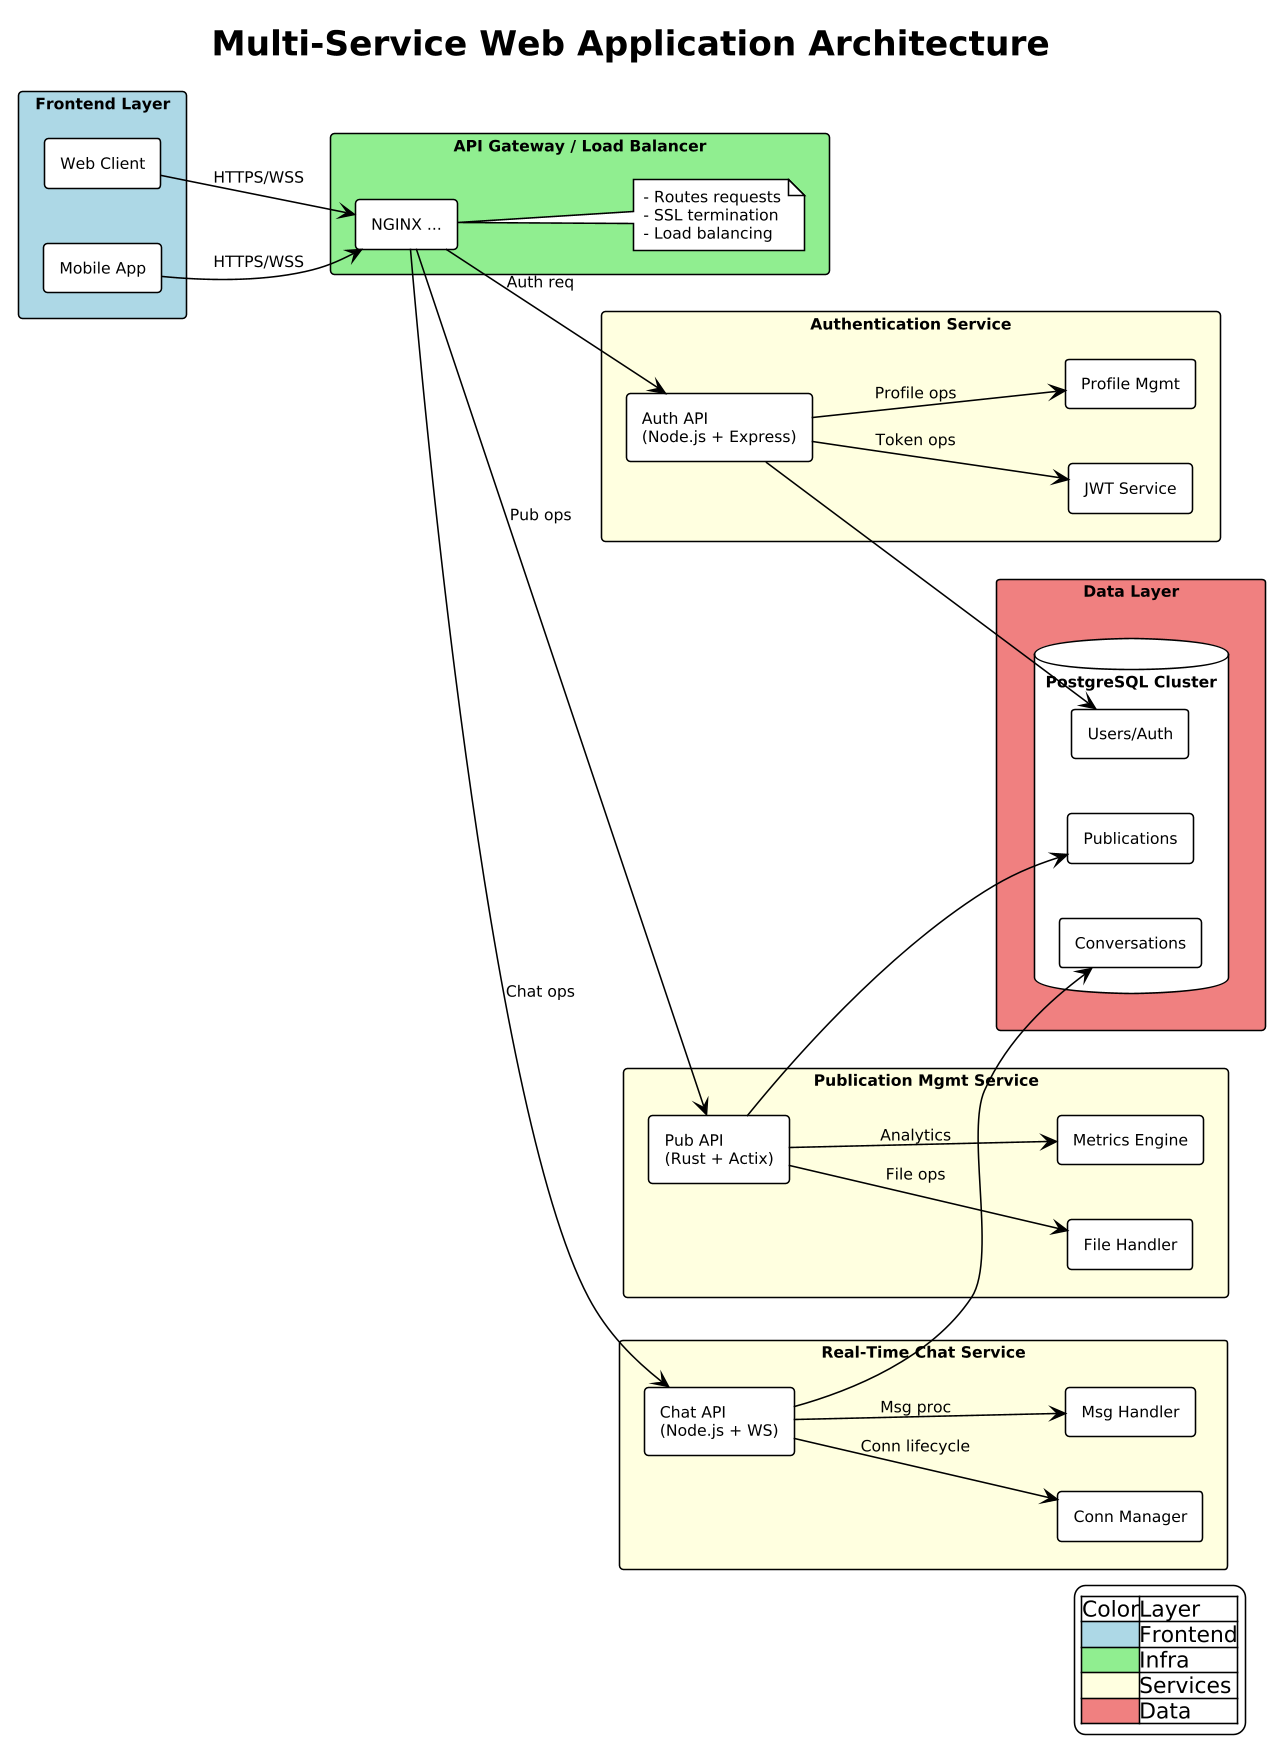
\includegraphics[width=0.8\textwidth]{diagrams/diagram.png}
    \caption{Diagramme général du système}
    \label{fig:diagram-general}
\end{figure}

\section{Diagramme 1}
\begin{figure}[htbp]
    \centering
    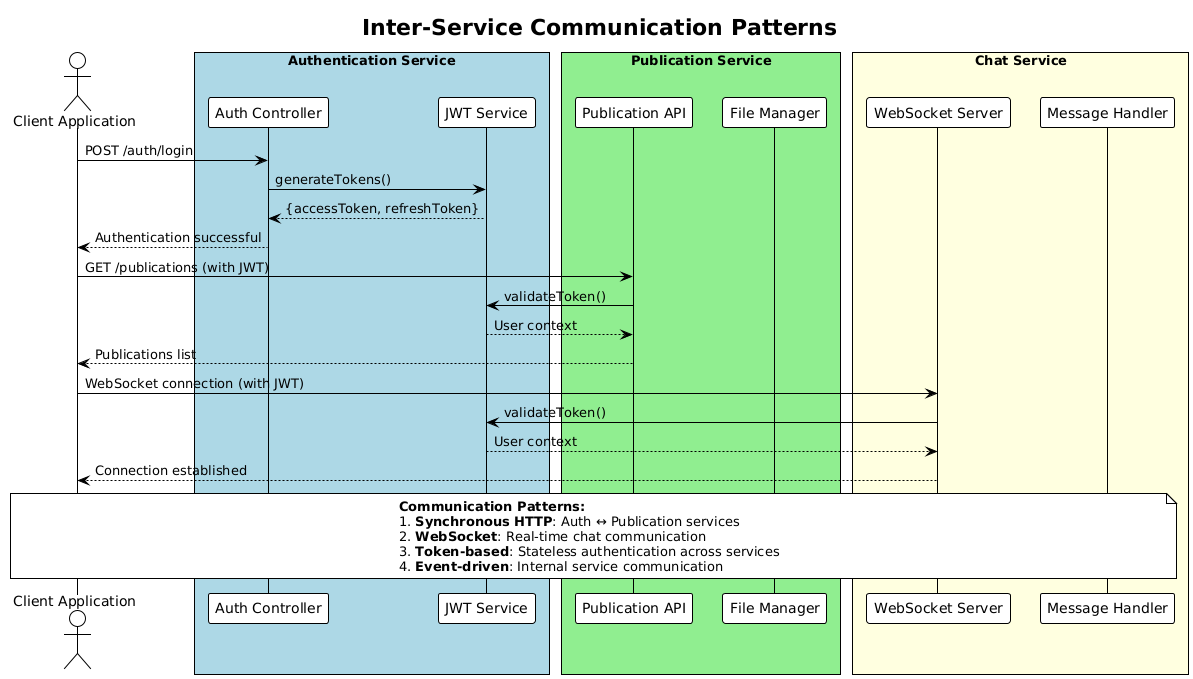
\includegraphics[width=0.8\textwidth]{diagrams/diagram1.png}
    \caption{Diagramme 1 - Description à compléter}
    \label{fig:diagram1}
\end{figure}

\section{Diagramme 2}
\begin{figure}[htbp]
    \centering
    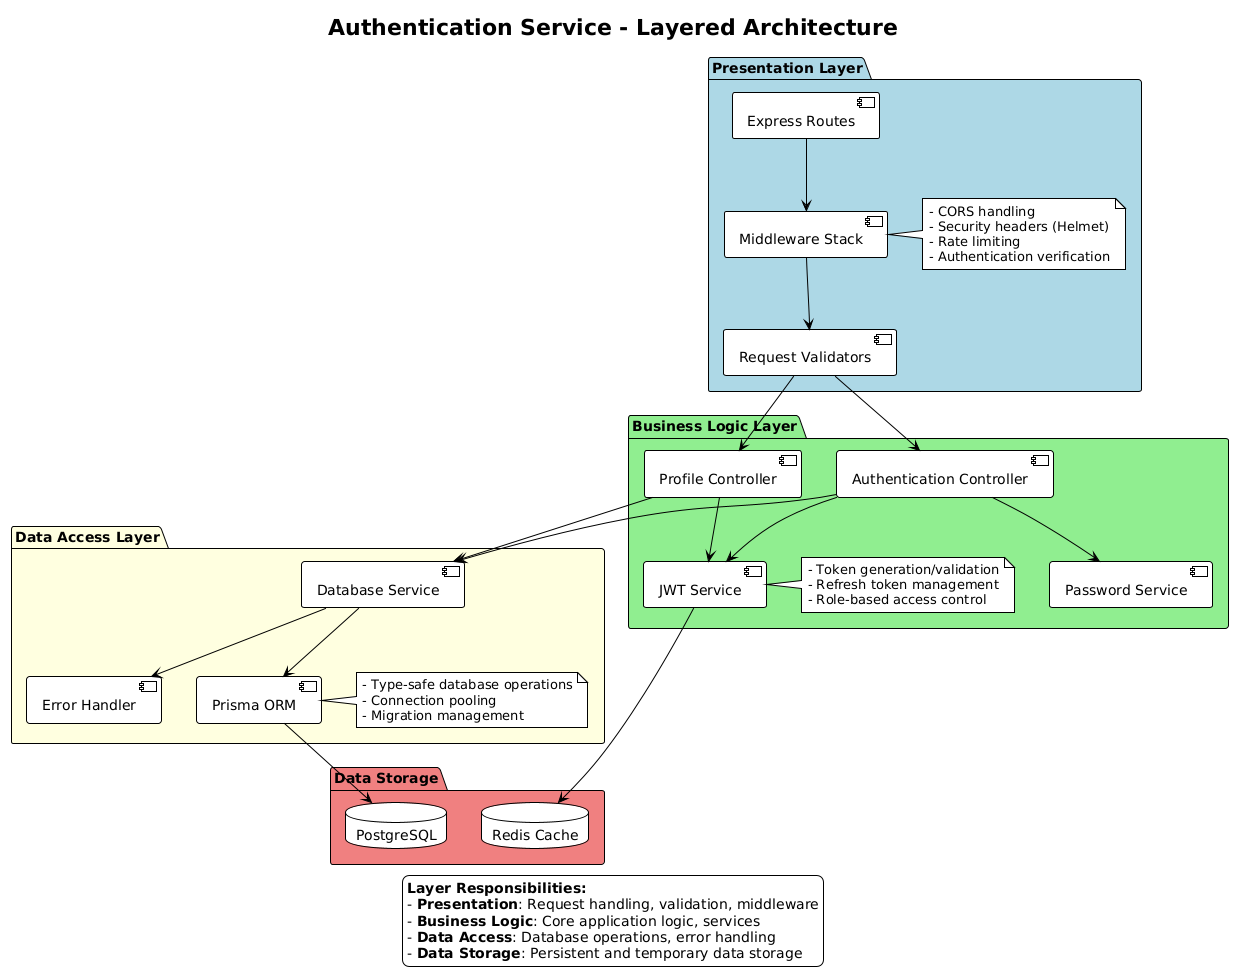
\includegraphics[width=0.8\textwidth]{diagrams/diagram2.png}
    \caption{Diagramme 2 - Description à compléter}
    \label{fig:diagram2}
\end{figure}

\section{Diagramme 3}
\begin{figure}[htbp]
    \centering
    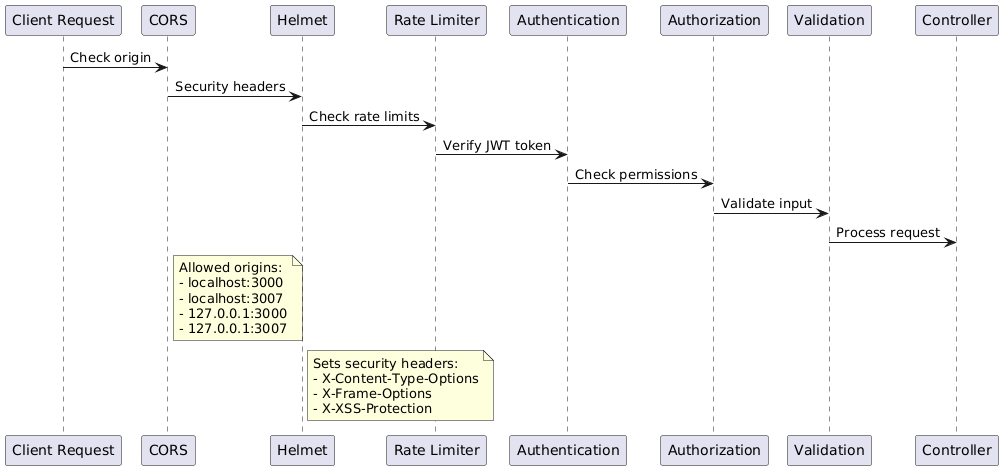
\includegraphics[width=0.8\textwidth]{diagrams/diagram3.png}
    \caption{Diagramme 3 - Description à compléter}
    \label{fig:diagram3}
\end{figure}

\section{Diagramme 4}
\begin{figure}[htbp]
    \centering
    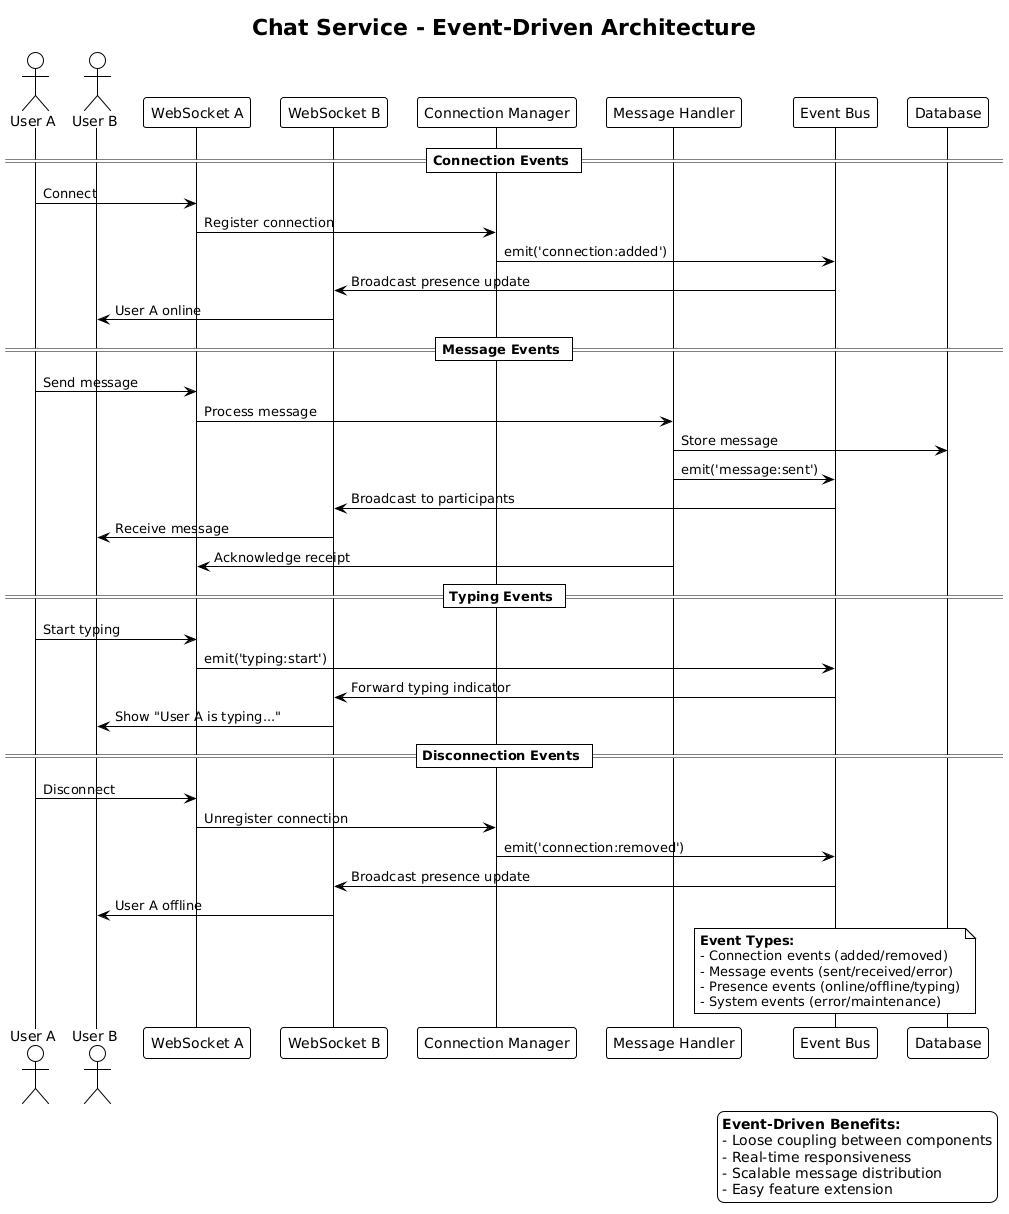
\includegraphics[width=0.8\textwidth]{diagrams/diagram4.png}
    \caption{Diagramme 4 - Description à compléter}
    \label{fig:diagram4}
\end{figure}

\section{Diagramme 5}
\begin{figure}[htbp]
    \centering
    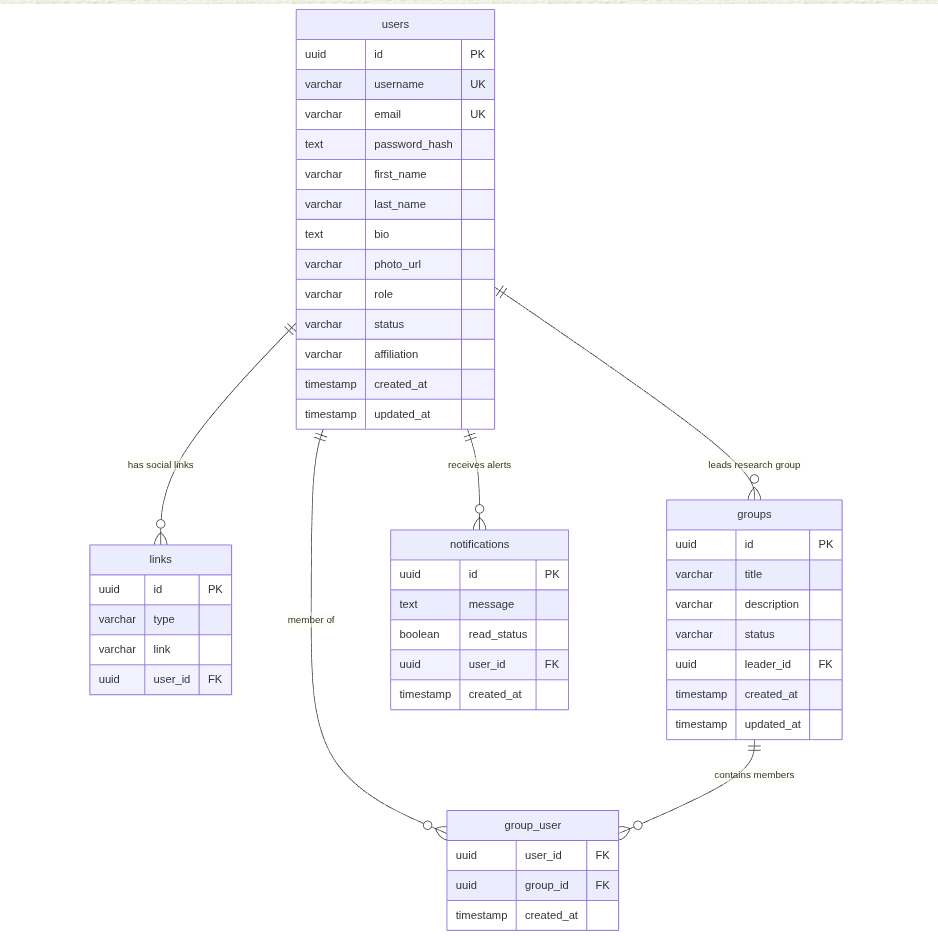
\includegraphics[width=0.8\textwidth]{diagrams/diagram5.png}
    \caption{Diagramme 5 - Description à compléter}
    \label{fig:diagram5}
\end{figure}

\section{Diagramme 6}
\begin{figure}[htbp]
    \centering
    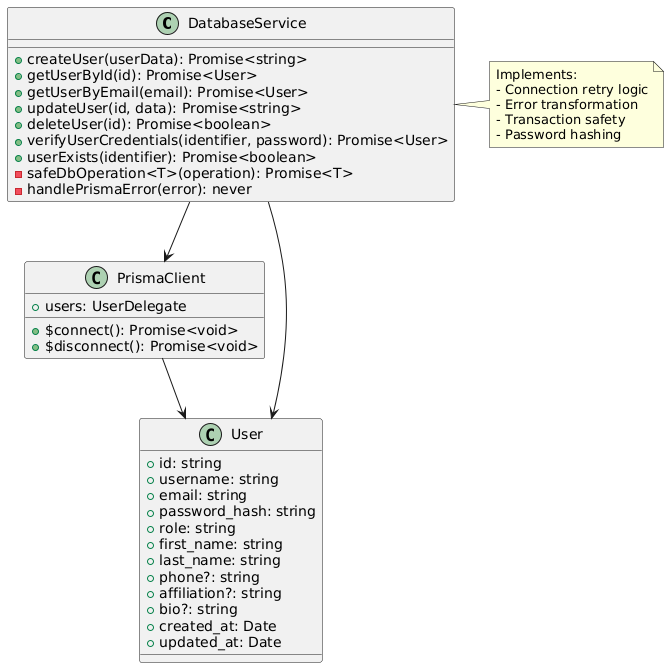
\includegraphics[width=0.8\textwidth]{diagrams/diagram6.png}
    \caption{Diagramme 6 - Description à compléter}
    \label{fig:diagram6}
\end{figure}

\section{Diagramme 7}
\begin{figure}[htbp]
    \centering
    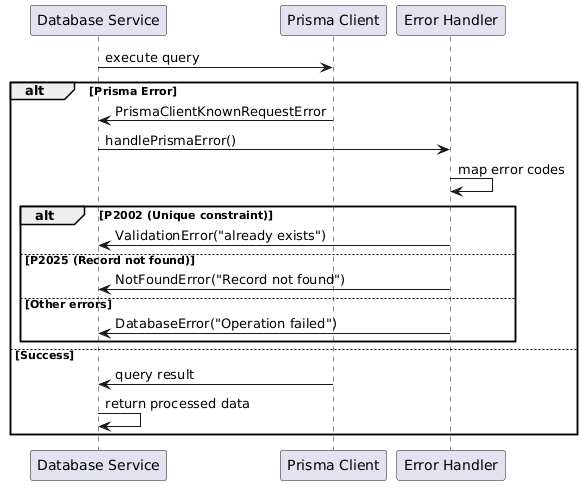
\includegraphics[width=0.8\textwidth]{diagrams/diagram7.png}
    \caption{Diagramme 7 - Description à compléter}
    \label{fig:diagram7}
\end{figure}

\section{Diagramme 8}
\begin{figure}[htbp]
    \centering
    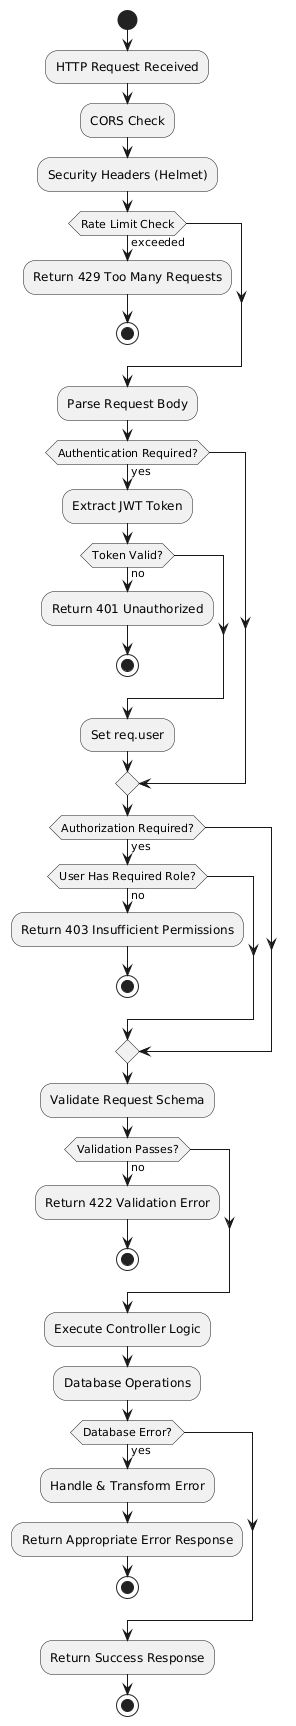
\includegraphics[width=0.8\textwidth]{diagrams/diagram8.png}
    \caption{Diagramme 8 - Description à compléter}
    \label{fig:diagram8}
\end{figure}

\section{Diagramme 9}
\begin{figure}[htbp]
    \centering
    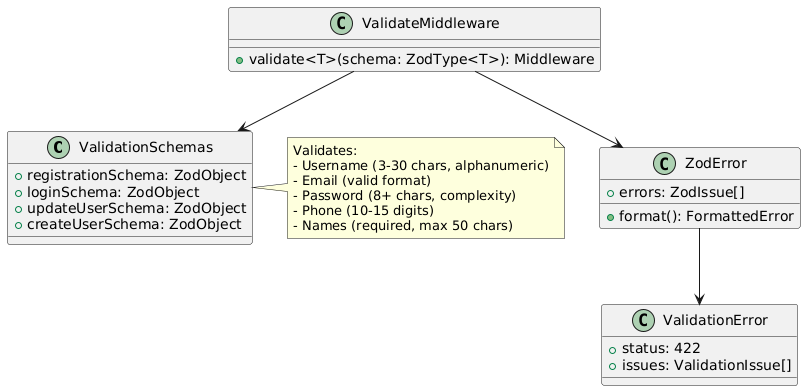
\includegraphics[width=0.8\textwidth]{diagrams/diagram9.png}
    \caption{Diagramme 9 - Description à compléter}
    \label{fig:diagram9}
\end{figure}

\section{Diagramme 10}
\begin{figure}[htbp]
    \centering
    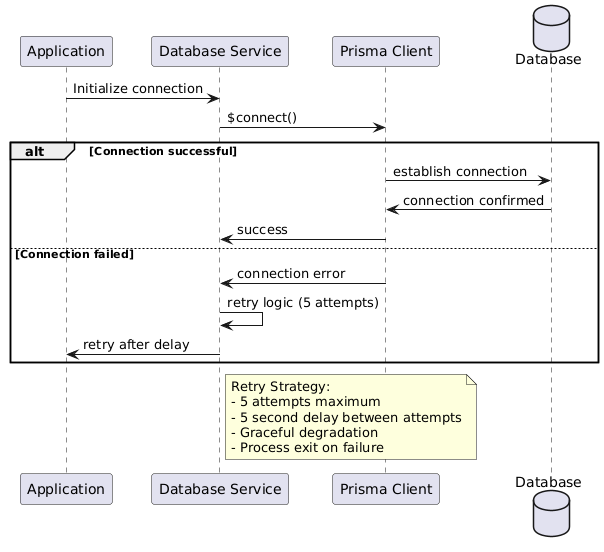
\includegraphics[width=0.8\textwidth]{diagrams/diagram10.png}
    \caption{Diagramme 10 - Description à compléter}
    \label{fig:diagram10}
\end{figure}

\section{Diagramme 11}
\begin{figure}[htbp]
    \centering
    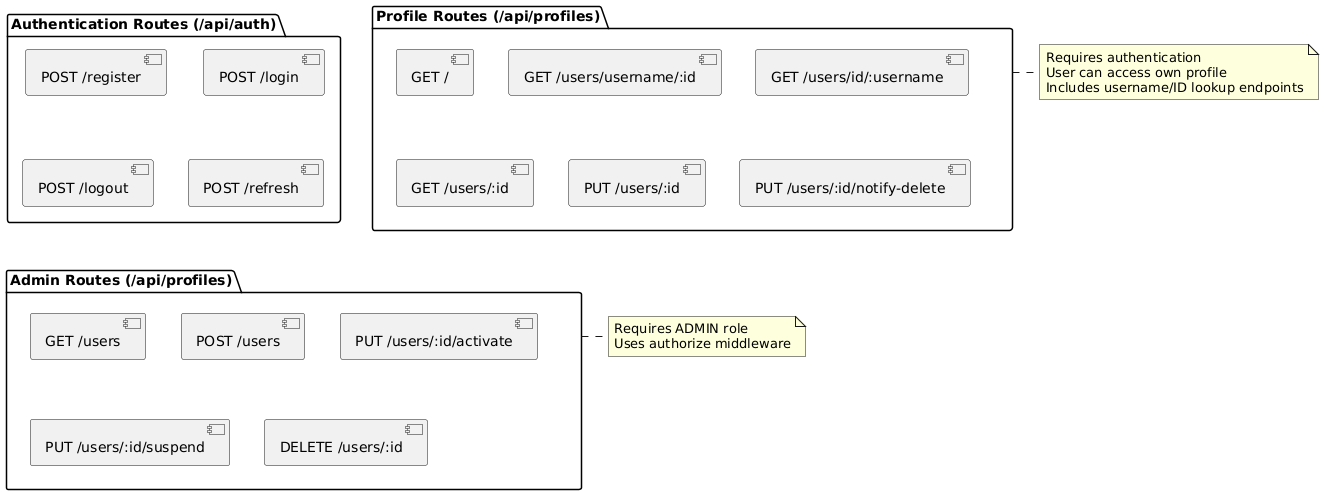
\includegraphics[width=0.8\textwidth]{diagrams/diagram11.png}
    \caption{Diagramme 11 - Description à compléter}
    \label{fig:diagram11}
\end{figure}

\section{Diagramme 12}
\begin{figure}[htbp]
    \centering
    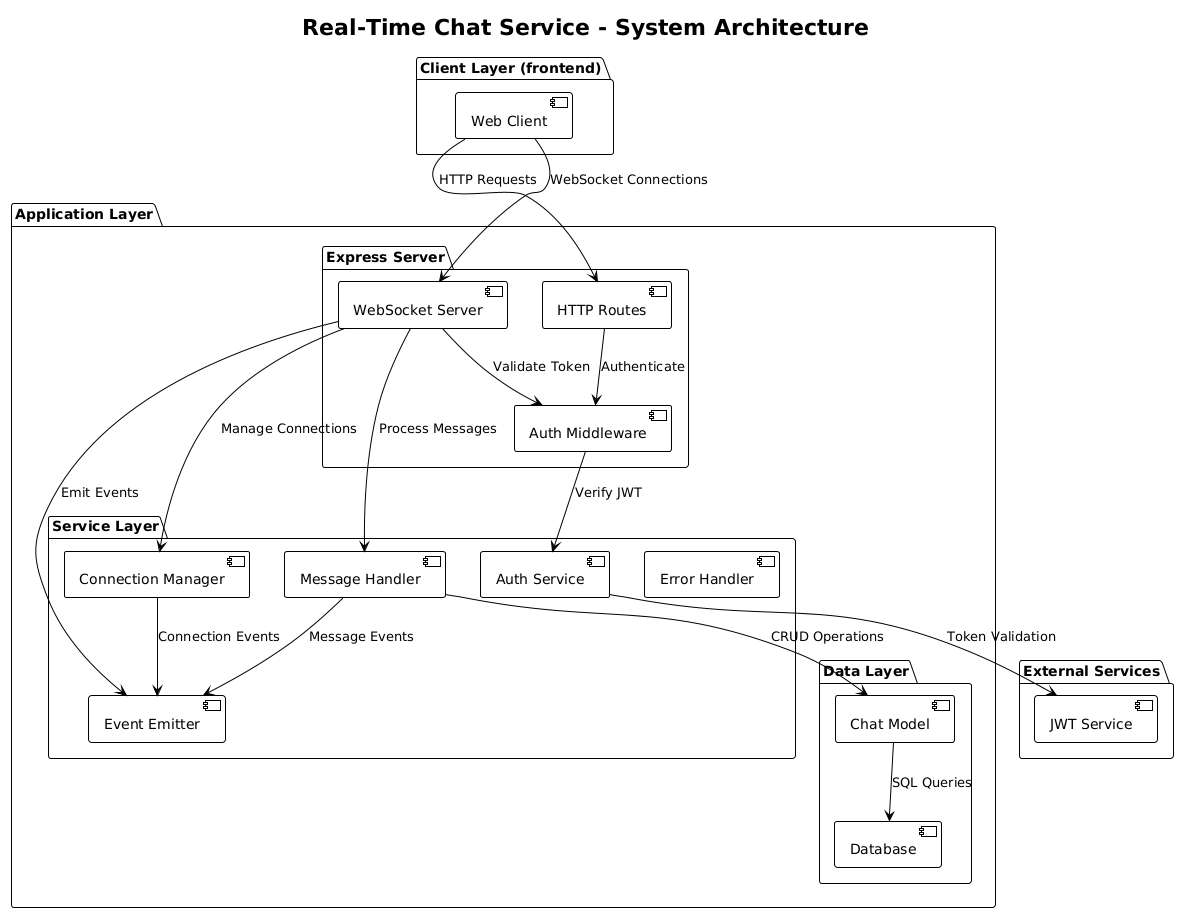
\includegraphics[width=0.8\textwidth]{diagrams/diagram12.png}
    \caption{Diagramme 12 - Description à compléter}
    \label{fig:diagram12}
\end{figure}

\section{Diagramme 13}
\begin{figure}[htbp]
    \centering
    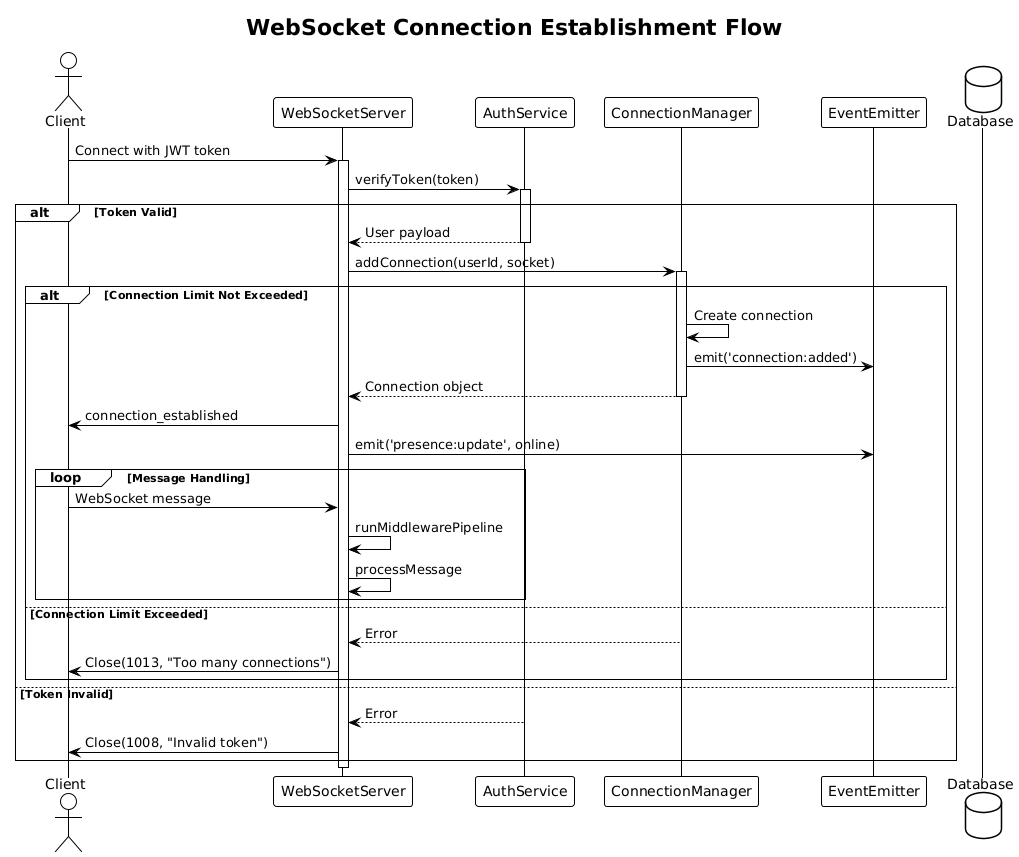
\includegraphics[width=0.8\textwidth]{diagrams/diagram13.png}
    \caption{Diagramme 13 - Description à compléter}
    \label{fig:diagram13}
\end{figure}

\section{Diagramme 14}
\begin{figure}[htbp]
    \centering
    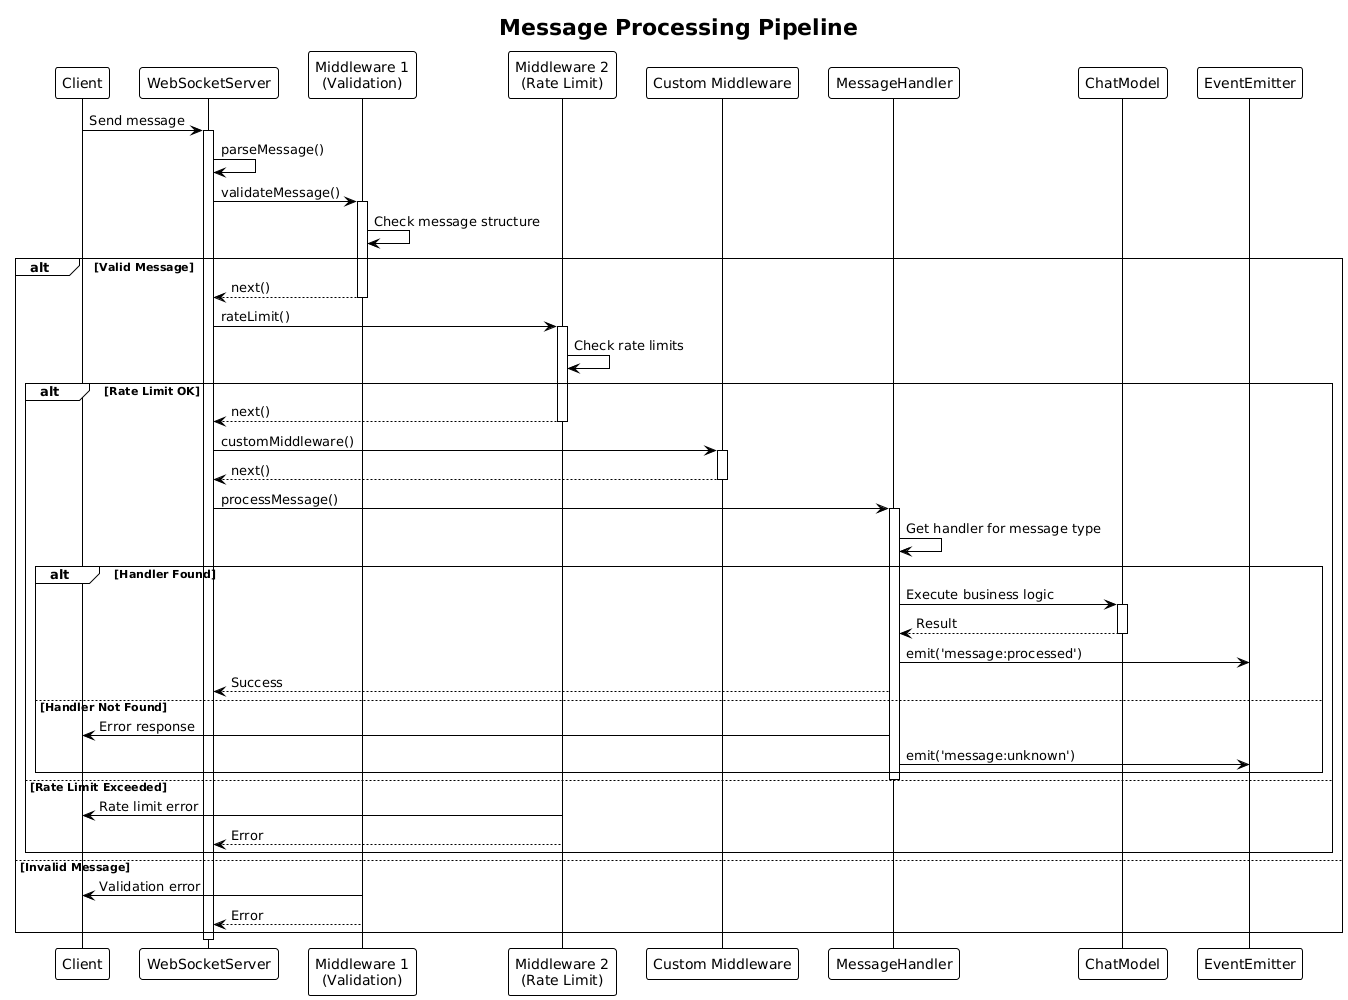
\includegraphics[width=0.8\textwidth]{diagrams/diagram14.png}
    \caption{Diagramme 14 - Description à compléter}
    \label{fig:diagram14}
\end{figure}

\section{Diagramme 15}
\begin{figure}[htbp]
    \centering
    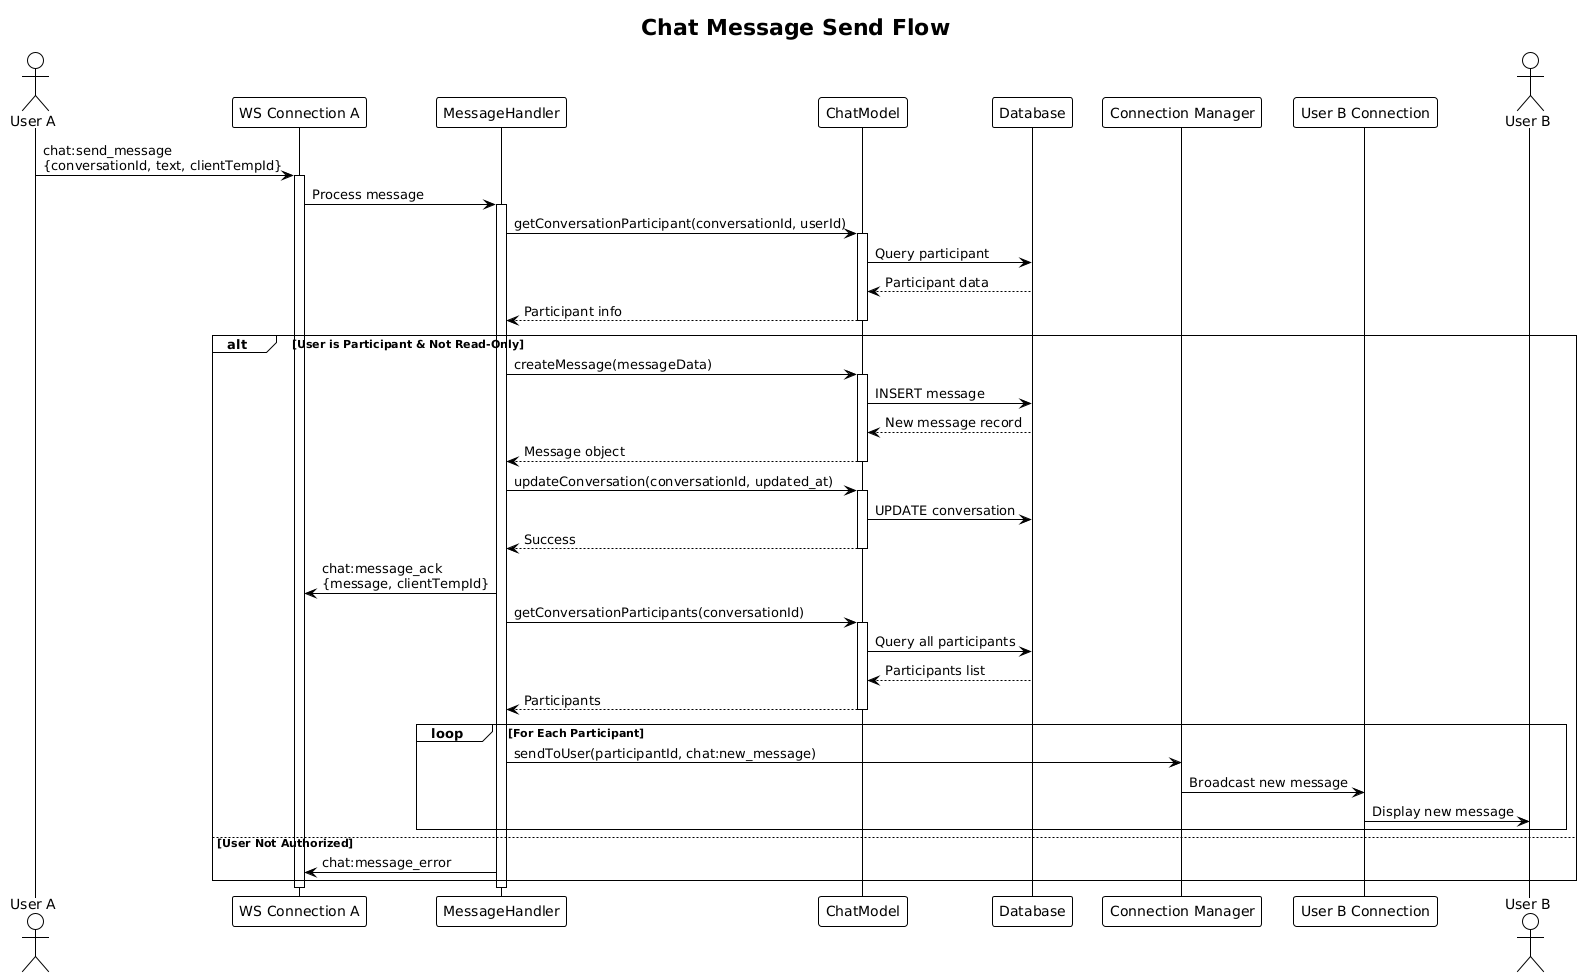
\includegraphics[width=0.8\textwidth]{diagrams/diagram15.png}
    \caption{Diagramme 15 - Description à compléter}
    \label{fig:diagram15}
\end{figure}


\section{Chat Database Schema}
\begin{figure}[htbp]
    \centering
    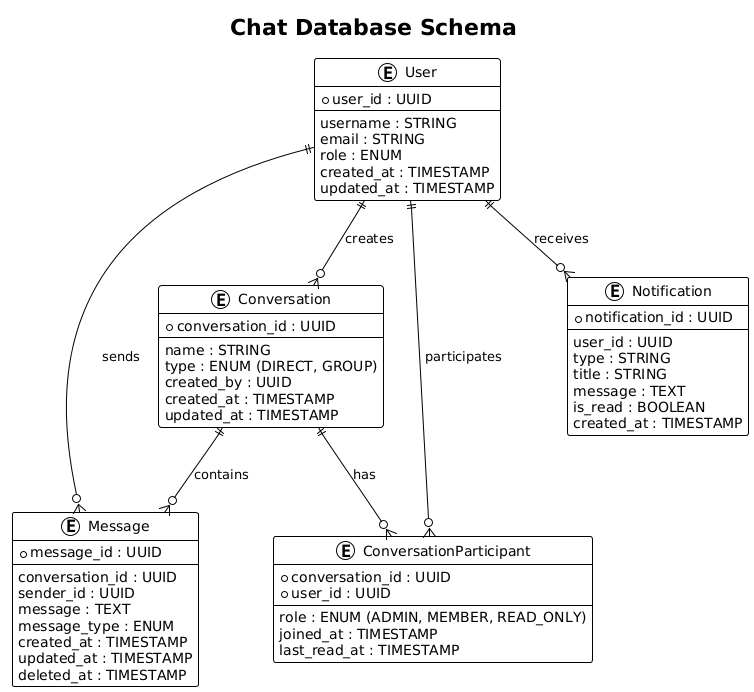
\includegraphics[width=0.8\textwidth]{diagrams/diagram18.png}
    \caption{Diagramme 18 - Description à compléter}
    \label{fig:diagram18}
\end{figure}

\section{Metrics and statistiques}
\begin{figure}[htbp]
    \centering
    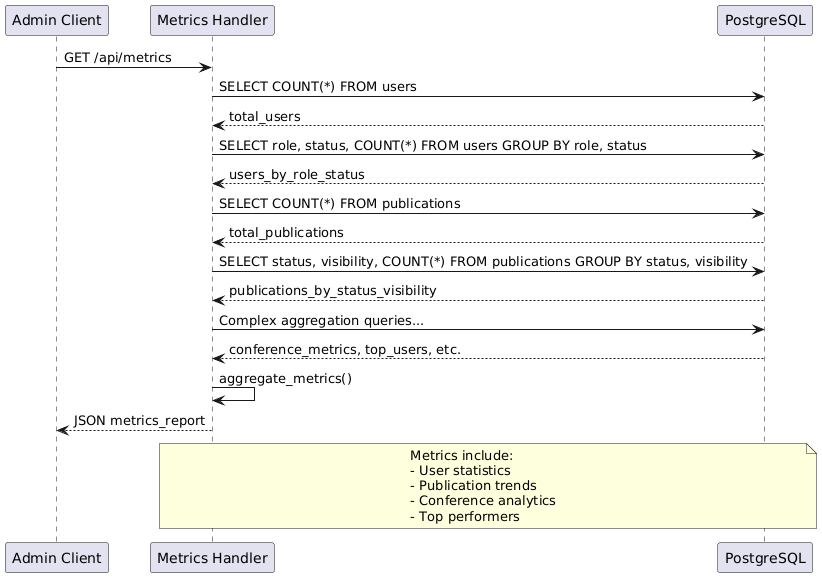
\includegraphics[width=0.8\textwidth]{diagrams/diagram19.png}
    \caption{Diagramme 19 - Description à compléter}
    \label{fig:diagram19}
\end{figure}

\section{Publications/Conference Workflow}
\begin{figure}[htbp]
    \centering
    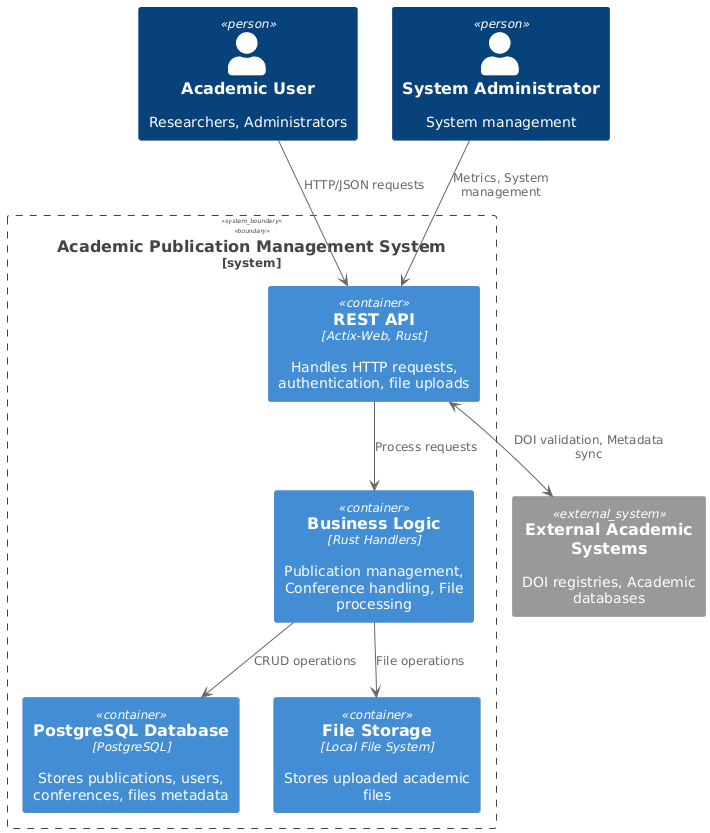
\includegraphics[width=0.8\textwidth]{diagrams/diagram20.png}
    \caption{Diagramme 20 - Description à compléter}
    \label{fig:diagram20}
\end{figure}

\section{Publications Lifecycle}
\begin{figure}[htbp]
    \centering
    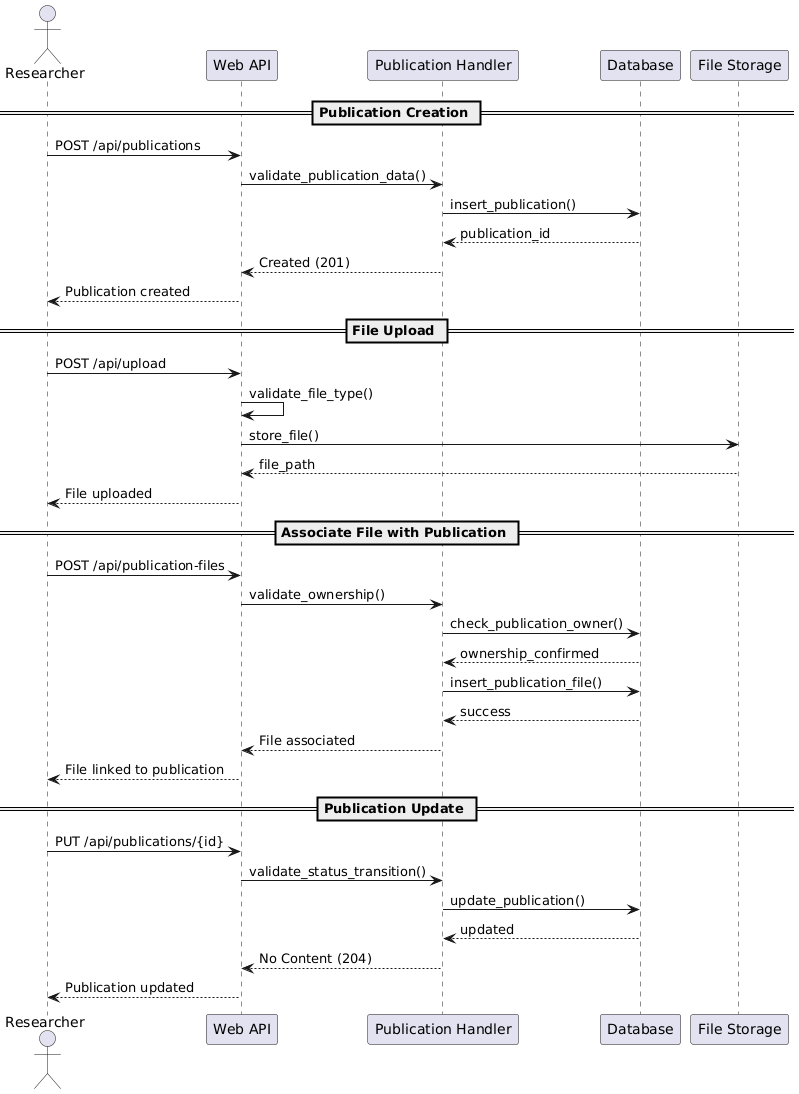
\includegraphics[width=0.8\textwidth]{diagrams/diagram21.png}
    \caption{Diagramme 21 - Description à compléter}
    \label{fig:diagram21}
\end{figure}

\section{Upload endpoint}
\begin{figure}[htbp]
    \centering
    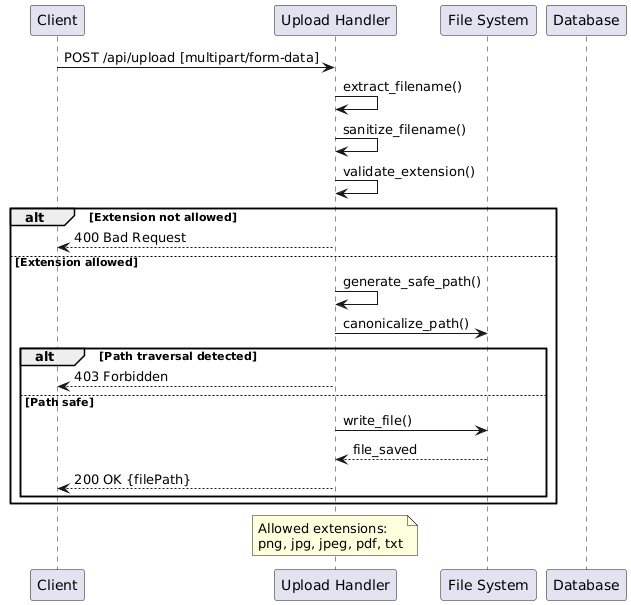
\includegraphics[width=0.8\textwidth]{diagrams/diagram22.png}
    \caption{Diagramme 22 - Description à compléter}
    \label{fig:diagram22}
\end{figure}


\section{Layered arch}
\begin{figure}[htbp]
    \centering
    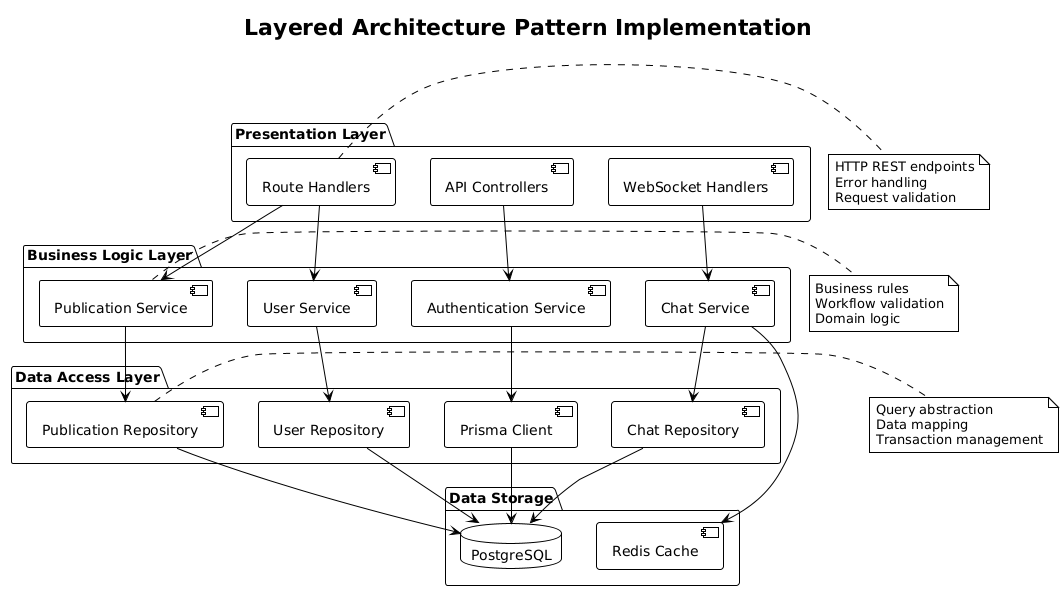
\includegraphics[width=0.8\textwidth]{diagrams/diagram24.png}
    \caption{Diagramme 24 - Description à compléter}
    \label{fig:diagram24}
\end{figure}


\section{Serivce interactions}
\begin{figure}[htbp]
    \centering
    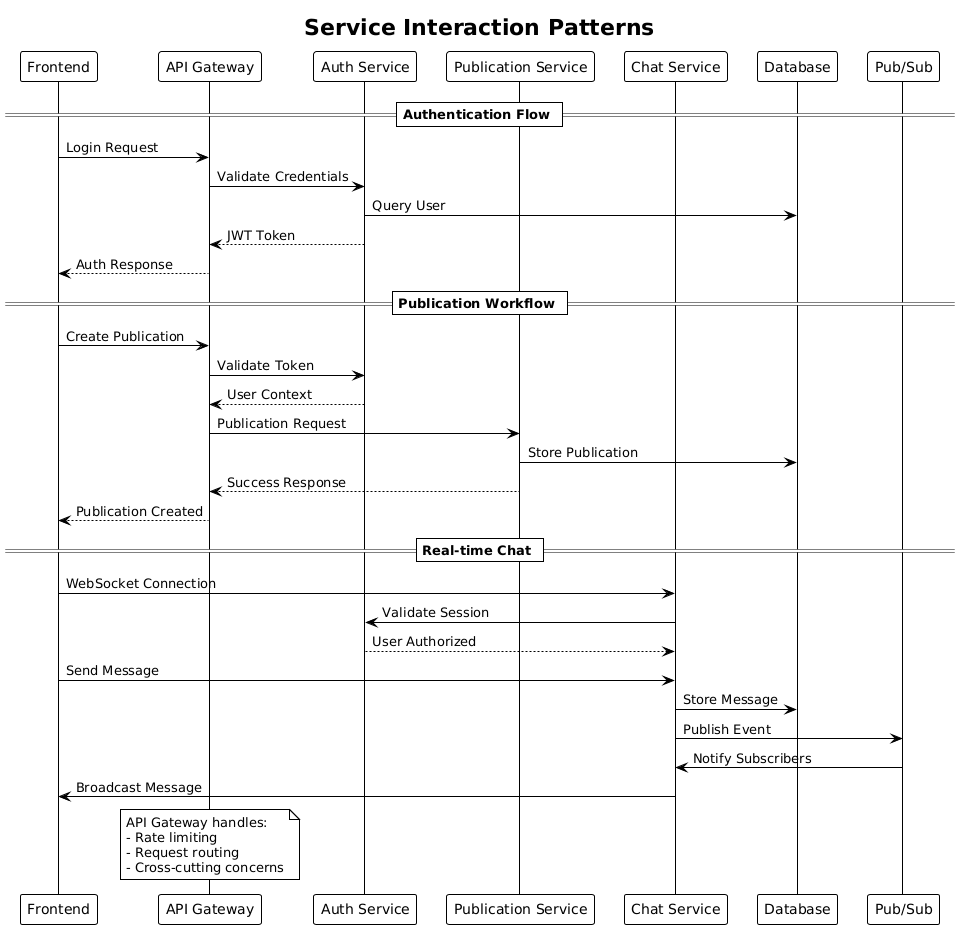
\includegraphics[width=0.8\textwidth]{diagrams/diagram26.png}
    \caption{Diagramme 26 - Description à compléter}
    \label{fig:diagram26}
\end{figure}

\section{Security Architecture}
\begin{figure}[htbp]
    \centering
    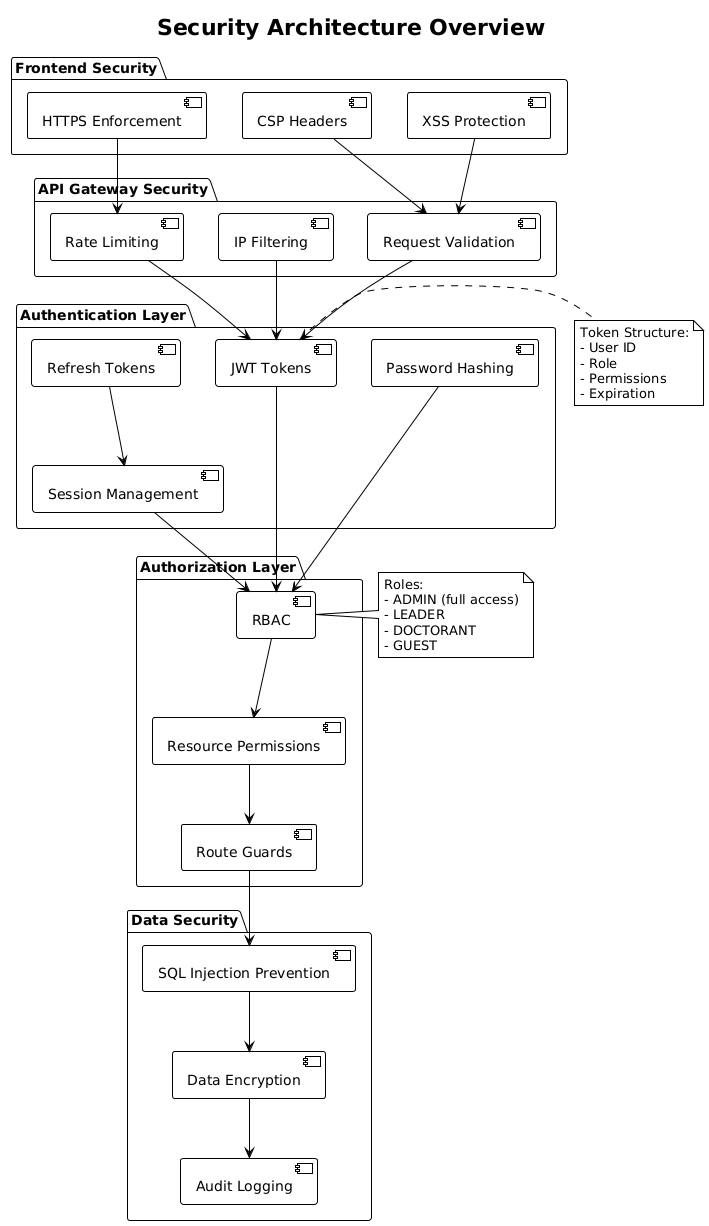
\includegraphics[width=0.8\textwidth]{diagrams/diagram27.png}
    \caption{Diagramme 27 - Description à compléter}
    \label{fig:diagram27}
\end{figure}

\newpage

\chapter{Mise en œuvre du site web}

\section{Gestion du code source et collaboration : GitHub}

Le choix de GitHub comme plateforme d’hébergement du code source et de collaboration a grandement contribué à industrialiser notre processus de développement, en alignant nos pratiques avec les standards professionnels actuels.

\subsection{Fonctionnalités stratégiques utilisées}

\begin{itemize}
    \item \textbf{Gestion des versions :} Chaque modification est tracée via des commits, assurant une traçabilité complète des évolutions du projet.
    \item \textbf{Travail collaboratif :} L’utilisation de branches dédiées et de pull requests permet à chaque développeur de travailler indépendamment tout en maintenant la stabilité de la branche principale.
    \item \textbf{Automatisation des validations :} L’intégration avec des outils externes permet l’exécution automatique de tests et de compilations avant toute fusion, garantissant ainsi la qualité du code.
\end{itemize}

\subsection{Organisation du dépôt et gestion des branches}

La branche \texttt{main} conserve la version stable du projet. Pour chaque nouvelle fonctionnalité ou correction, une branche spécifique est créée. Cette organisation minimise les conflits et favorise un développement parallèle efficace.

\subsection{Demandes de fusion et revue de code}

Les pull requests assurent une revue rigoureuse du code par les membres de l’équipe, permettant la détection précoce d’erreurs, l’amélioration de la qualité du code, ainsi que le partage des connaissances.

\subsection{Suivi des tâches avec GitHub Issues}

GitHub Issues a été employé pour documenter et prioriser les tâches. Chaque problème ou nouvelle fonctionnalité fait l’objet d’une issue, facilitant la planification et le suivi de l’avancement.

\subsection{Impact global de GitHub}

Cette méthodologie a permis de centraliser le développement, faciliter le travail asynchrone, maintenir un historique détaillé des modifications, et renforcer la rigueur grâce aux revues systématiques.

\section{Tests des API : Postman}

Postman a été l’outil principal pour tester, documenter et valider les API RESTful développées. Ses fonctionnalités clés incluent :

\begin{itemize}
    \item \textbf{Environnements configurables} pour gérer les différentes phases (développement, production).
    \item \textbf{Collections organisées} permettant de regrouper les endpoints et de faciliter leur réutilisation.
    \item \textbf{Tests automatisés} écrits en JavaScript, garantissant la conformité des réponses (statut, format, performance).
    \item \textbf{Documentation dynamique} générée automatiquement pour faciliter l’intégration frontend/backend.
\end{itemize}

\section{Tests des WebSockets : wscat}

Pour valider les fonctionnalités temps réel telles que les notifications ou le chat, l’outil en ligne de commande \texttt{wscat} a été utilisé :

\begin{itemize}
    \item Connexion directe aux serveurs WebSocket pour envoyer et recevoir des messages en temps réel.
    \item Tests de stabilité et de latence, permettant un débogage efficace.
    \item Facilité d’intégration dans des scripts automatisés grâce à sa compatibilité shell.
\end{itemize}

\section{Gestion et interrogation des bases de données : DBeaver}

DBeaver a permis une gestion centralisée des bases de données du projet, notamment PostgreSQL, grâce à :

\begin{itemize}
    \item Un éditeur SQL puissant avec coloration syntaxique et auto-complétion.
    \item Une visualisation claire des schémas, tables, relations et index.
    \item Des fonctionnalités d’import/export pour manipuler facilement les données.
    \item La gestion sécurisée des connexions (SSH, SSL) pour protéger l’accès aux données.
\end{itemize}

\section{Conteneurisation et orchestration : Docker}

Docker a été un pilier de notre mise en œuvre, assurant la cohérence des environnements de développement et de tests.

\subsection{Mise en œuvre technique}

\begin{itemize}
    \item Utilisation de \texttt{Dockerfiles} pour définir des images reproductibles des services backend, frontend et base de données.
    \item Orchestration avec \texttt{Docker Compose} pour gérer le lancement simultané et les dépendances entre conteneurs.
    \item Volumes persistants configurés pour assurer la durabilité des données malgré la recréation des conteneurs.
\end{itemize}

\subsection{Bénéfices}

\begin{itemize}
    \item Isolation stricte des environnements pour éviter les conflits de dépendances.
    \item Portabilité permettant une exécution identique en local, en staging et en production.
    \item Préparation facilitée à la scalabilité et à l’intégration future avec Kubernetes.
    \item Intégration possible avec GitHub Actions pour automatiser les builds et tests continus.
\end{itemize}

\section{Synthèse}

Cette phase de mise en œuvre a permis d’établir une base solide pour le développement du site web, en s’appuyant sur des outils et méthodes professionnels garantissant qualité, traçabilité et collaboration efficace. Bien que le déploiement en production ne soit pas encore réalisé, toutes les préparations nécessaires ont été intégrées dès cette étape afin de faciliter cette future étape.


% ... Répétez pour diagram3.png à diagram27.png ...
\newpage
\chapter*{Conclusion Générale}
\addcontentsline{toc}{chapter}{Conclusion Générale}
Ce projet s’inscrit dans une volonté d’améliorer la gestion des activités de recherche à travers une plateforme centralisée. Grâce à une architecture moderne basée sur des microservices, une base de données PostgreSQL, une interface intuitive et une sécurité renforcée, l’application répond aux besoins croissants des laboratoires universitaires. Les perspectives d’évolution incluent l’intégration d’outils analytiques avancés et l’extension vers d’autres structures de recherche.

\newpage
\bibliographystyle{plain}
\bibliography{refs}

\newpage
\chapter*{Annexes}
\addcontentsline{toc}{chapter}{Annexes}
% Ajouter vos annexes ici

\end{document}
